% COSC 267 HCI Final Project Presentation
% AI Learning Coach Lab - Three Interaction Paradigms

\documentclass[aspectratio=169]{beamer}

% Theme and Color Scheme
\usetheme{Madrid}
\usecolortheme{seahorse}

% Packages
\usepackage{graphicx}
\usepackage{booktabs}
\usepackage{tikz}
\usepackage{fontawesome5}
\usepackage{xcolor}
\usepackage{hyperref}

% Custom colors matching the web app
\definecolor{defaultColor}{RGB}{107, 114, 128}
\definecolor{coCreationColor}{RGB}{59, 130, 246}
\definecolor{explainableColor}{RGB}{245, 158, 11}
\definecolor{accentColor}{RGB}{102, 126, 234}

% Title Information
\title[AI Learning Coach Lab]{AI Learning Coach Lab}
\subtitle{Exploring Three Human-AI Interaction Paradigms}
\author{Yujin Tang (f007yh4) \and Jun Jie Ou Yang (f0080w9)}
\institute{COSC 267 - Human-Computer Interaction\\Dartmouth College}
\date{\today}

% Footer
\setbeamertemplate{footline}[frame number]

\begin{document}

% Title Slide
\begin{frame}
\titlepage
\end{frame}

% Table of Contents
\begin{frame}{Outline}
\tableofcontents
\end{frame}

% ============================================================
\section{Introduction}
% ============================================================

\begin{frame}{Project Overview}
\begin{columns}
\column{0.5\textwidth}
\textbf{What is this project?}
\begin{itemize}
    \item Interactive web application
    \item Three AI learning coach prototypes
    \item Comparative HCI research
    \item Built with React + TypeScript
\end{itemize}

\vspace{0.5cm}
\textbf{Why this matters?}
\begin{itemize}
    \item AI systems are increasingly prevalent
    \item User interaction design is critical
    \item Trade-offs between control \& automation
\end{itemize}

\column{0.5\textwidth}
\begin{center}
\begin{tikzpicture}
    \node[circle, fill=defaultColor!30, minimum size=2cm] at (0,2) {\faRobot};
    \node[circle, fill=coCreationColor!30, minimum size=2cm] at (-1.5,0) {\faHandshake};
    \node[circle, fill=explainableColor!30, minimum size=2cm] at (1.5,0) {\faLightbulb};
    \draw[->, thick] (0,1.5) -- (-1.2,0.5);
    \draw[->, thick] (0,1.5) -- (1.2,0.5);
\end{tikzpicture}
\end{center}
\end{columns}
\end{frame}

\begin{frame}{Research Context}
\begin{block}{Central Question}
How do different AI interaction paradigms affect user experience, trust, and learning outcomes?
\end{block}

\vspace{0.3cm}

\begin{columns}
\column{0.33\textwidth}
\centering
\textcolor{defaultColor}{\textbf{User Autonomy}}
\\[0.2cm]
How much control should users have?

\column{0.33\textwidth}
\centering
\textcolor{coCreationColor}{\textbf{Transparency}}
\\[0.2cm]
Should AI explain its decisions?

\column{0.33\textwidth}
\centering
\textcolor{explainableColor}{\textbf{Cognitive Load}}
\\[0.2cm]
What's the right balance?
\end{columns}

\vspace{0.5cm}

\begin{alertblock}{Our Approach}
Implement three distinct prototypes representing different points on the automation-transparency-control spectrum
\end{alertblock}
\end{frame}

\begin{frame}{Project Scope}
\begin{columns}
\column{0.6\textwidth}
\textbf{Technical Implementation:}
\begin{itemize}
    \item \textbf{45 learning activities} across 3 math topics
    \item \textbf{180+ practice problems} with hints \& solutions
    \item Algebra, Functions, and Limits
    \item Multiple difficulty levels (Easy, Medium, Hard)
    \item Time estimates: 10-45 minutes per activity
    \item Responsive, modern UI design
\end{itemize}

\vspace{0.3cm}
\textbf{Interaction Design:}
\begin{itemize}
    \item Three fundamentally different approaches
    \item Real-time, interactive prototypes
    \item Rich content for meaningful demonstrations
    \item Production-ready web application
\end{itemize}

\column{0.4\textwidth}
\begin{center}
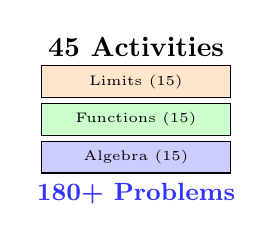
\begin{tikzpicture}[scale=0.8]
    % Database visualization
    \draw[fill=blue!20] (0,0) rectangle (3,0.5) node[pos=.5] {\tiny Algebra (15)};
    \draw[fill=green!20] (0,0.6) rectangle (3,1.1) node[pos=.5] {\tiny Functions (15)};
    \draw[fill=orange!20] (0,1.2) rectangle (3,1.7) node[pos=.5] {\tiny Limits (15)};
    \node[above] at (1.5,1.7) {\textbf{45 Activities}};
    \node[below] at (1.5,0) {\small \textcolor{blue!80}{\textbf{180+ Problems}}};
\end{tikzpicture}
\end{center}

\vspace{0.3cm}
\begin{exampleblock}{Live Demo}
\centering
\texttt{localhost:5173}
\end{exampleblock}
\end{columns}
\end{frame}

% ============================================================
\section{Three Prototypes}
% ============================================================

\begin{frame}{Prototype Comparison Overview}
\begin{table}
\centering
\small
\begin{tabular}{l|ccc}
\toprule
\textbf{Aspect} & \textcolor{defaultColor}{\textbf{Default}} & \textcolor{coCreationColor}{\textbf{Co-Creation}} & \textcolor{explainableColor}{\textbf{Explainable}} \\
\midrule
User Control & \faTimesCircle{} Low & \faCheckCircle{} High & \faCheck{} Medium \\
Transparency & \faTimesCircle{} None & \faCheck{} Process & \faCheckCircle{} Full \\
Cognitive Load & \faCheckCircle{} Minimal & \faCheck{} Medium & \faTimes{} Higher \\
Decision Speed & \faCheckCircle{} Fast & \faTimes{} Slow & \faCheck{} Medium \\
Personalization & \faTimesCircle{} None & \faCheckCircle{} High & \faCheck{} Medium \\
Trust Building & \faTimes{} Implicit & \faCheck{} Active & \faCheckCircle{} Explicit \\
\bottomrule
\end{tabular}
\end{table}

\vspace{0.3cm}
\begin{center}
\textit{Each prototype represents a different philosophy in human-AI collaboration}
\end{center}
\end{frame}

% -------------------- Default Path --------------------
\begin{frame}{Prototype 1: Default Path}
\begin{columns}
\column{0.5\textwidth}
\begin{block}{\faRobot{} Traditional AI Recommendation}
The baseline approach - AI makes all decisions
\end{block}

\vspace{0.3cm}
\textbf{Key Features:}
\begin{itemize}
    \item AI automatically recommends activities
    \item \textcolor{blue!80}{\textbf{Shows all practice problems}} with hints
    \item Binary choice: Accept or Reject
    \item Minimal user input required
    \item History tracking
    \item Fast and efficient
\end{itemize}

\vspace{0.3cm}
\textbf{Design Philosophy:}
\begin{quote}
\textit{"The AI knows best - just trust the algorithm"}
\end{quote}

\column{0.5\textwidth}
\begin{center}
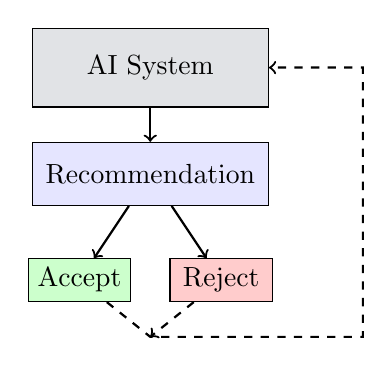
\begin{tikzpicture}[scale=0.9]
    % Flow diagram
    \node[rectangle, draw, fill=defaultColor!20, minimum width=3cm, minimum height=1cm] (ai) at (0,3) {AI System};
    \node[rectangle, draw, fill=blue!10, minimum width=3cm, minimum height=0.8cm] (rec) at (0,1.5) {Recommendation};
    \node[rectangle, draw, fill=green!20, minimum width=1.3cm] (accept) at (-1,0) {Accept};
    \node[rectangle, draw, fill=red!20, minimum width=1.3cm] (reject) at (1,0) {Reject};
    
    \draw[->, thick] (ai) -- (rec);
    \draw[->, thick] (rec) -- (accept);
    \draw[->, thick] (rec) -- (reject);
    \draw[->, thick, dashed] (accept) -- (0,-0.8) -- (3,-0.8) -- (3,3) -- (ai);
    \draw[->, thick, dashed] (reject) -- (0,-0.8);
\end{tikzpicture}
\end{center}

\vspace{0.3cm}
\textbf{Use Case:}
\\Quick decisions, expert users, high trust in AI
\end{columns}
\end{frame}

\begin{frame}{Default Path: Strengths \& Weaknesses}
\begin{columns}
\column{0.5\textwidth}
\begin{block}{Advantages \faThumbsUp}
\begin{itemize}
    \item \textcolor{green!70!black}{\textbf{Efficiency:}} Fastest interaction
    \item \textcolor{green!70!black}{\textbf{Simplicity:}} Minimal cognitive load
    \item \textcolor{green!70!black}{\textbf{Automation:}} No preference setting needed
    \item \textcolor{green!70!black}{\textbf{Scalability:}} Works with any content
\end{itemize}
\end{block}

\column{0.5\textwidth}
\begin{alertblock}{Limitations \faExclamationTriangle}
\begin{itemize}
    \item \textcolor{red!70!black}{\textbf{No Control:}} Users can't express preferences
    \item \textcolor{red!70!black}{\textbf{Black Box:}} No reasoning visible
    \item \textcolor{red!70!black}{\textbf{Trust Issues:}} Blind faith required
    \item \textcolor{red!70!black}{\textbf{Frustration:}} May recommend irrelevant items
\end{itemize}
\end{alertblock}
\end{columns}

\vspace{0.5cm}
\begin{exampleblock}{Real-World Examples}
Netflix auto-play, YouTube recommendations, Amazon "You might like..."
\end{exampleblock}
\end{frame}

% -------------------- Co-Creation Path --------------------
\begin{frame}{Prototype 2: Co-Creation Path}
\begin{columns}
\column{0.5\textwidth}
\begin{block}{\faHandshake{} Collaborative Decision Making}
User and AI work together to create learning plans
\end{block}

\vspace{0.2cm}
\textbf{Key Features:}
\begin{itemize}
    \item Users set preferences (topic, difficulty, time)
    \item AI generates multiple recommendations
    \item \textcolor{blue!80}{\textbf{Click to reveal practice problems}}
    \item Users select from options
    \item Flexible, personalized results
    \item Real-time filtering
\end{itemize}

\vspace{0.2cm}
\textbf{Design Philosophy:}
\\[0.1cm]
\textit{"Let's decide together - you know yourself best"}

\column{0.5\textwidth}
\begin{center}
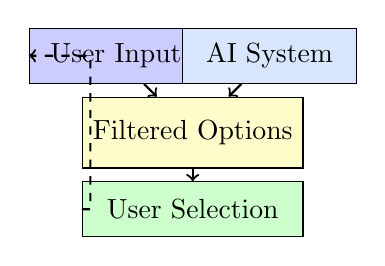
\begin{tikzpicture}[scale=0.65]
    % Collaborative flow
    \node[rectangle, draw, fill=blue!20, minimum width=2.2cm, minimum height=0.7cm] (user) at (-1.5,3) {User Input};
    \node[rectangle, draw, fill=coCreationColor!20, minimum width=2.2cm, minimum height=0.7cm] (ai) at (1.5,3) {AI System};
    \node[rectangle, draw, fill=yellow!20, minimum width=2.8cm, minimum height=0.9cm] (filter) at (0,1.5) {Filtered Options};
    \node[rectangle, draw, fill=green!20, minimum width=2.8cm, minimum height=0.7cm] (select) at (0,0) {User Selection};
    
    \draw[->, thick] (user) -- (filter);
    \draw[->, thick] (ai) -- (filter);
    \draw[->, thick] (filter) -- (select);
    \draw[->, thick, dashed] (select) -- (-2,0) -- (-2,3) -- (user);
\end{tikzpicture}
\end{center}

\vspace{0.3cm}
\textbf{Use Case:}
\\Personalized learning, diverse needs, user empowerment
\end{columns}
\end{frame}

\begin{frame}{Co-Creation Path: Strengths \& Weaknesses}
\begin{columns}
\column{0.5\textwidth}
\begin{block}{Advantages \faThumbsUp}
\begin{itemize}
    \item \textcolor{green!70!black}{\textbf{Control:}} User agency and autonomy
    \item \textcolor{green!70!black}{\textbf{Personalization:}} Matches user needs
    \item \textcolor{green!70!black}{\textbf{Flexibility:}} Multiple options available
    \item \textcolor{green!70!black}{\textbf{Engagement:}} Active participation
\end{itemize}
\end{block}

\column{0.5\textwidth}
\begin{alertblock}{Limitations \faExclamationTriangle}
\begin{itemize}
    \item \textcolor{red!70!black}{\textbf{Effort:}} Requires user input
    \item \textcolor{red!70!black}{\textbf{Time:}} Slower than default
    \item \textcolor{red!70!black}{\textbf{Complexity:}} More decisions to make
    \item \textcolor{red!70!black}{\textbf{Bias:}} Users might limit themselves
\end{itemize}
\end{alertblock}
\end{columns}

\vspace{0.5cm}
\begin{exampleblock}{Real-World Examples}
Spotify's filter options, Amazon's advanced search, course selection systems
\end{exampleblock}
\end{frame}

% -------------------- Explainable Path --------------------
\begin{frame}{Prototype 3: Explainable Path}
\begin{columns}
\column{0.5\textwidth}
\begin{block}{\faLightbulb{} Transparent AI Decision Making}
AI explains its reasoning and shows confidence
\end{block}

\vspace{0.2cm}
\textbf{Key Features:}
\begin{itemize}
    \item AI recommendations with explanations
    \item \textcolor{blue!80}{\textbf{Preview first 3 problems}} (+ more indicator)
    \item Multiple reasoning types
    \item Confidence metrics visualization
    \item Database statistics (includes 180+ problems)
    \item Toggle-able transparency
\end{itemize}

\vspace{0.2cm}
\textbf{Design Philosophy:}
\\[0.1cm]
\textit{"Here's what I recommend and why - you decide"}

\column{0.5\textwidth}
\begin{center}
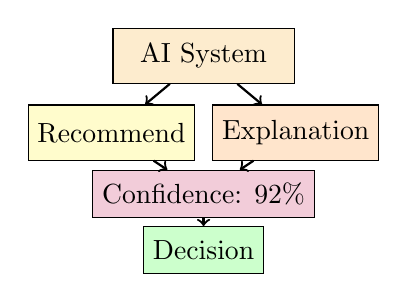
\begin{tikzpicture}[scale=0.65]
    % Explainable flow
    \node[rectangle, draw, fill=explainableColor!20, minimum width=2.3cm, minimum height=0.7cm] (ai) at (0,3.5) {AI System};
    \node[rectangle, draw, fill=yellow!20, minimum width=2.0cm, minimum height=0.7cm] (rec) at (-1.8,2) {Recommend};
    \node[rectangle, draw, fill=orange!20, minimum width=2.0cm, minimum height=0.7cm] (exp) at (1.8,2) {Explanation};
    \node[rectangle, draw, fill=purple!20, minimum width=2.8cm, minimum height=0.6cm] (conf) at (0,0.8) {Confidence: 92\%};
    \node[rectangle, draw, fill=green!20, minimum width=1.5cm, minimum height=0.6cm] (accept) at (0,-0.3) {Decision};
    
    \draw[->, thick] (ai) -- (rec);
    \draw[->, thick] (ai) -- (exp);
    \draw[->, thick] (rec) -- (conf);
    \draw[->, thick] (exp) -- (conf);
    \draw[->, thick] (conf) -- (accept);
\end{tikzpicture}
\end{center}

\vspace{0.3cm}
\textbf{Use Case:}
\\High-stakes decisions, building trust, learning
\end{columns}
\end{frame}

\begin{frame}{Explainable Path: Strengths \& Weaknesses}
\begin{columns}
\column{0.5\textwidth}
\begin{block}{Advantages \faThumbsUp}
\begin{itemize}
    \item \textcolor{green!70!black}{\textbf{Transparency:}} Full decision visibility
    \item \textcolor{green!70!black}{\textbf{Trust:}} Builds informed confidence
    \item \textcolor{green!70!black}{\textbf{Education:}} Users learn AI logic
    \item \textcolor{green!70!black}{\textbf{Debugging:}} Easy to spot errors
\end{itemize}
\end{block}

\column{0.5\textwidth}
\begin{alertblock}{Limitations \faExclamationTriangle}
\begin{itemize}
    \item \textcolor{red!70!black}{\textbf{Complexity:}} More information to process
    \item \textcolor{red!70!black}{\textbf{Cognitive Load:}} Can be overwhelming
    \item \textcolor{red!70!black}{\textbf{Time:}} Slower decision making
    \item \textcolor{red!70!black}{\textbf{Over-trust:}} May blindly follow "science"
\end{itemize}
\end{alertblock}
\end{columns}

\vspace{0.5cm}
\begin{exampleblock}{Real-World Examples}
LIME/SHAP in ML, Google Search snippets, medical diagnosis systems
\end{exampleblock}
\end{frame}

% ============================================================
\section{Comparative Analysis}
% ============================================================

\begin{frame}{Design Trade-offs}
\begin{center}
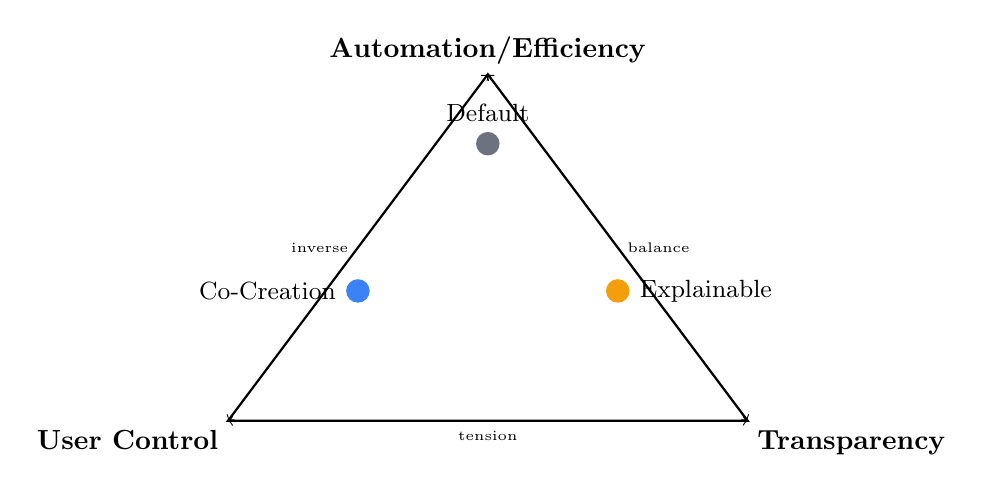
\begin{tikzpicture}[scale=1.1]
    % Triangle of trade-offs
    \coordinate (A) at (0,4);
    \coordinate (B) at (-3,0);
    \coordinate (C) at (3,0);
    
    \draw[thick] (A) -- (B) -- (C) -- cycle;
    
    \node[above] at (A) {\textbf{Automation/Efficiency}};
    \node[below left] at (B) {\textbf{User Control}};
    \node[below right] at (C) {\textbf{Transparency}};
    
    % Prototypes positioned
    \node[circle, fill=defaultColor, inner sep=3pt, label=above:{\small Default}] at (0,3.2) {};
    \node[circle, fill=coCreationColor, inner sep=3pt, label=left:{\small Co-Creation}] at (-1.5,1.5) {};
    \node[circle, fill=explainableColor, inner sep=3pt, label=right:{\small Explainable}] at (1.5,1.5) {};
    
    % Arrows showing trade-offs
    \draw[<->, dashed] (A) -- node[left] {\tiny inverse} (B);
    \draw[<->, dashed] (B) -- node[below] {\tiny tension} (C);
    \draw[<->, dashed] (C) -- node[right] {\tiny balance} (A);
\end{tikzpicture}
\end{center}

\textbf{Key Insight:} No single "best" design - depends on context and user needs
\end{frame}

\begin{frame}{User Experience Dimensions}
\begin{table}
\centering
\begin{tabular}{p{3cm}|p{3cm}|p{3cm}|p{3cm}}
\toprule
\textbf{Dimension} & \textbf{\textcolor{defaultColor}{Default}} & \textbf{\textcolor{coCreationColor}{Co-Creation}} & \textbf{\textcolor{explainableColor}{Explainable}} \\
\midrule
\textbf{User Agency} & Passive recipient & Active collaborator & Informed decision-maker \\[0.3cm]
\textbf{Trust Model} & Implicit trust & Earned through control & Built via transparency \\[0.3cm]
\textbf{Error Recovery} & Reject \& retry & Re-filter options & Understand \& adjust \\[0.3cm]
\textbf{Learning Curve} & Minimal & Moderate & Steeper \\
\bottomrule
\end{tabular}
\end{table}
\end{frame}

\begin{frame}{When to Use Each Prototype?}
\begin{columns}
\column{0.33\textwidth}
\begin{block}{\textcolor{defaultColor}{Default Path}}
\textbf{Best for:}
\begin{itemize}
    \item Quick decisions
    \item Routine tasks
    \item Expert users
    \item High AI trust
    \item Low stakes
\end{itemize}

\vspace{0.2cm}
\textbf{Examples:}
\begin{itemize}
    \item Music playlists
    \item News feeds
    \item Product suggestions
\end{itemize}
\end{block}

\column{0.33\textwidth}
\begin{block}{\textcolor{coCreationColor}{Co-Creation}}
\textbf{Best for:}
\begin{itemize}
    \item Personalized needs
    \item Diverse preferences
    \item User empowerment
    \item Flexible goals
    \item Medium stakes
\end{itemize}

\vspace{0.2cm}
\textbf{Examples:}
\begin{itemize}
    \item Course selection
    \item Travel planning
    \item Shopping filters
\end{itemize}
\end{block}

\column{0.33\textwidth}
\begin{block}{\textcolor{explainableColor}{Explainable}}
\textbf{Best for:}
\begin{itemize}
    \item High-stakes decisions
    \item Building trust
    \item Learning contexts
    \item Accountability
    \item Medical/Legal
\end{itemize}

\vspace{0.2cm}
\textbf{Examples:}
\begin{itemize}
    \item Medical diagnosis
    \item Loan approvals
    \item Legal systems
\end{itemize}
\end{block}
\end{columns}
\end{frame}

% ============================================================
\section{Research Questions}
% ============================================================

\begin{frame}{Primary Research Questions}
\begin{enumerate}
    \item \textbf{User Preference:} Which interaction paradigm do users prefer and why?
    
    \vspace{0.3cm}
    \item \textbf{Task Performance:} Does the interface design affect learning outcomes?
    
    \vspace{0.3cm}
    \item \textbf{Trust \& Satisfaction:} How does transparency impact user trust?
    
    \vspace{0.3cm}
    \item \textbf{Cognitive Load:} What is the optimal balance between information and simplicity?
    
    \vspace{0.3cm}
    \item \textbf{Context Dependency:} Do preferences change based on task difficulty or user expertise?
\end{enumerate}
\end{frame}

\begin{frame}{Potential User Study Design}
\begin{block}{Within-Subjects Design}
Each participant uses all three prototypes with different learning activities
\end{block}

\vspace{0.3cm}

\textbf{Metrics to Measure:}
\begin{itemize}
    \item \textbf{Quantitative:} Task completion time, number of interactions, success rate
    \item \textbf{Qualitative:} User satisfaction, perceived control, trust ratings
    \item \textbf{Behavioral:} Navigation patterns, preference expressions, error recovery
\end{itemize}

\vspace{0.3cm}

\begin{alertblock}{Hypothesis}
Transparency and control increase user satisfaction, but may slow decision-making. The optimal design depends on task context and user expertise.
\end{alertblock}
\end{frame}

% ============================================================
\section{Technical Implementation}
% ============================================================

\begin{frame}{System Architecture}
\begin{columns}
\column{0.6\textwidth}
\textbf{Technology Stack:}
\begin{itemize}
    \item \textbf{Frontend:} React 18 + TypeScript
    \item \textbf{Build Tool:} Vite 4
    \item \textbf{Styling:} CSS-in-JS (inline styles)
    \item \textbf{State Management:} React Hooks
    \item \textbf{Data:} Client-side (45 activities, 180+ problems)
\end{itemize}

\vspace{0.3cm}
\textbf{Key Features:}
\begin{itemize}
    \item Single-page application (SPA)
    \item Responsive design
    \item No backend required
    \item Production-ready
    \item Deployable to Vercel/Netlify
\end{itemize}

\column{0.4\textwidth}
\begin{center}
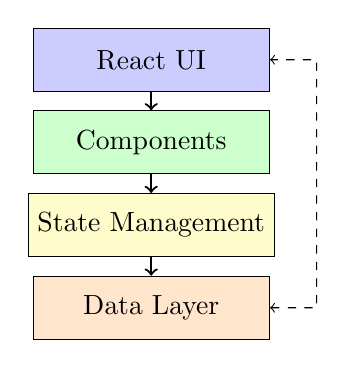
\begin{tikzpicture}[scale=0.7]
    \node[rectangle, draw, fill=blue!20, minimum width=3cm, minimum height=0.8cm] (ui) at (0,4) {React UI};
    \node[rectangle, draw, fill=green!20, minimum width=3cm, minimum height=0.8cm] (comp) at (0,2.5) {Components};
    \node[rectangle, draw, fill=yellow!20, minimum width=3cm, minimum height=0.8cm] (state) at (0,1) {State Management};
    \node[rectangle, draw, fill=orange!20, minimum width=3cm, minimum height=0.8cm] (data) at (0,-0.5) {Data Layer};
    
    \draw[->, thick] (ui) -- (comp);
    \draw[->, thick] (comp) -- (state);
    \draw[->, thick] (state) -- (data);
    \draw[<->, dashed] (data) -- (3,-0.5) -- (3,4) -- (ui);
\end{tikzpicture}
\end{center}

\vspace{0.3cm}
\texttt{localhost:5173}
\end{columns}
\end{frame}

\begin{frame}[fragile]{Code Quality \& Scalability}
\begin{columns}
\column{0.5\textwidth}
\textbf{Best Practices:}
\begin{itemize}
    \item Type-safe TypeScript
    \item Component-based architecture
    \item Modular data structure
    \item Clean separation of concerns
    \item Consistent styling
\end{itemize}

\vspace{0.3cm}
\textbf{File Structure:}
\begin{verbatim}
src/
|-- components/
|   |-- DefaultPath.tsx
|   |-- CoCreationPath.tsx
|   |-- ExplainablePath.tsx
|-- data/
|   |-- activities.ts
|       (45 activities, 180+ exercises)
|-- types.ts (Activity, Exercise)
|-- App.tsx
\end{verbatim}

\column{0.5\textwidth}
\textbf{Extensibility:}
\begin{itemize}
    \item Easy to add new activities
    \item Simple to create new prototypes
    \item Configurable recommendation algorithm
    \item Scalable to other domains
\end{itemize}

\vspace{0.3cm}
\begin{exampleblock}{Future Enhancements}
\begin{itemize}
    \item User authentication
    \item Progress tracking
    \item Analytics dashboard
    \item A/B testing framework
    \item Backend integration
\end{itemize}
\end{exampleblock}
\end{columns}
\end{frame}

% ============================================================
\section{Demonstration}
% ============================================================

\begin{frame}{Live Demo Structure}
\begin{center}
\Large \textbf{Time for a Live Demonstration!}
\end{center}

\vspace{0.5cm}

\begin{enumerate}
    \item \textbf{Default Path (2 min):}
    \begin{itemize}
        \item Show quick accept/reject flow
        \item \textcolor{blue!80}{View all practice problems with hints}
        \item Demonstrate history tracking
        \item Highlight lack of control
    \end{itemize}
    
    \vspace{0.3cm}
    \item \textbf{Co-Creation Path (3 min):}
    \begin{itemize}
        \item Set preferences (topics, difficulty, time)
        \item Generate filtered recommendations
        \item \textcolor{blue!80}{Click activities to reveal problems}
        \item Select multiple activities
        \item Show personalization power
    \end{itemize}
    
    \vspace{0.3cm}
    \item \textbf{Explainable Path (3 min):}
    \begin{itemize}
        \item \textcolor{blue!80}{Preview first 3 practice problems}
        \item View AI explanations
        \item Examine confidence metrics
        \item Toggle transparency
        \item Show database statistics (180+ problems)
    \end{itemize}
\end{enumerate}
\end{frame}

\begin{frame}{Demo Scenarios}
\begin{block}{Scenario 1: Time-Constrained Student}
\textit{"I only have 20 minutes and want to review easy Algebra topics"}
\\[0.2cm]
\textbf{Best fit:} Co-Creation Path (filter by time + topic + difficulty)
\end{block}

\vspace{0.3cm}

\begin{block}{Scenario 2: Curious Learner}
\textit{"I want to understand why the AI recommends this particular topic"}
\\[0.2cm]
\textbf{Best fit:} Explainable Path (shows reasoning + confidence)
\end{block}

\vspace{0.3cm}

\begin{block}{Scenario 3: Quick Review}
\textit{"Just give me something to practice, I trust the system"}
\\[0.2cm]
\textbf{Best fit:} Default Path (fast, minimal interaction)
\end{block}
\end{frame}

% ============================================================
\section{Conclusion}
% ============================================================

\begin{frame}{Key Takeaways}
\begin{enumerate}
    \item \textbf{No Universal Best Design}
    \begin{itemize}
        \item Context matters
        \item User expertise varies
        \item Task complexity influences preference
    \end{itemize}
    
    \vspace{0.3cm}
    \item \textbf{Trade-offs Are Inherent}
    \begin{itemize}
        \item Automation vs. Control
        \item Simplicity vs. Transparency
        \item Speed vs. Understanding
    \end{itemize}
    
    \vspace{0.3cm}
    \item \textbf{Human-Centered AI Design}
    \begin{itemize}
        \item Put users in control when appropriate
        \item Provide transparency when needed
        \item Balance efficiency with agency
    \end{itemize}
\end{enumerate}
\end{frame}

\begin{frame}{Future Work \& Extensions}
\begin{columns}
\column{0.5\textwidth}
\textbf{Research Directions:}
\begin{itemize}
    \item Conduct user studies
    \item Measure learning outcomes
    \item Test with diverse populations
    \item Explore hybrid approaches
    \item Analyze long-term effects
\end{itemize}

\vspace{0.3cm}
\textbf{Technical Enhancements:}
\begin{itemize}
    \item Machine learning integration
    \item Adaptive recommendations
    \item Real-time analytics
    \item Multi-user support
\end{itemize}

\column{0.5\textwidth}
\textbf{Domain Extensions:}
\begin{itemize}
    \item Other academic subjects
    \item Professional training
    \item Healthcare recommendations
    \item Financial planning
    \item Career guidance
\end{itemize}

\vspace{0.3cm}
\begin{alertblock}{Impact}
This framework can inform design decisions for any AI-powered recommendation system
\end{alertblock}
\end{columns}
\end{frame}

\begin{frame}{Project Impact \& Contributions}
\begin{block}{HCI Contributions}
\begin{itemize}
    \item Concrete instantiation of three interaction paradigms
    \item Production-quality implementation for testing
    \item Foundation for empirical research
    \item Educational tool for understanding AI transparency
\end{itemize}
\end{block}

\vspace{0.3cm}

\begin{block}{Broader Implications}
\begin{itemize}
    \item Informs AI ethics discussions
    \item Supports explainable AI movement
    \item Promotes user-centered design
    \item Demonstrates practical trade-offs
\end{itemize}
\end{block}

\vspace{0.3cm}

\begin{center}
\textit{Good AI design requires understanding both technology AND human needs}
\end{center}
\end{frame}

% Final slide
\begin{frame}[plain]
\begin{center}
{\Huge Thank You!}

\vspace{1cm}

{\Large Questions \& Discussion}

\vspace{1cm}

\texttt{Demo: localhost:5173}

\vspace{0.5cm}

\small
COSC 267 - Human-Computer Interaction\\
Dartmouth College
\end{center}
\end{frame}

% Backup slides
\appendix

\begin{frame}[allowframebreaks]{References \& Resources}
\begin{thebibliography}{9}
\bibitem{norman2013}
Norman, D. (2013). \textit{The Design of Everyday Things: Revised and Expanded Edition}. Basic Books.

\bibitem{shneiderman2016}
Shneiderman, B. (2016). The dangers of faulty, biased, or malicious algorithms requires independent oversight. \textit{Proceedings of the National Academy of Sciences}.

\bibitem{miller2019}
Miller, T. (2019). Explanation in artificial intelligence: Insights from the social sciences. \textit{Artificial Intelligence}, 267, 1-38.

\bibitem{amershi2019}
Amershi, S., et al. (2019). Guidelines for human-AI interaction. \textit{CHI Conference on Human Factors in Computing Systems}.

\bibitem{guidotti2018}
Guidotti, R., et al. (2018). A survey of methods for explaining black box models. \textit{ACM Computing Surveys}, 51(5), 1-42.
\end{thebibliography}
\end{frame}

\end{document}

